\documentclass[journal]{IEEEtran}
\usepackage{fontspec}
\setmainfont{Times New Roman}
\setsansfont{Arial}
\usepackage{amsmath,amssymb,graphicx,booktabs,tabularx,array,url}
\usepackage[hidelinks]{hyperref}\usepackage{microtype}
\setlength{\emergencystretch}{2em}
\newcommand{\Range}{\operatorname{Range}}
\title{When Should a Receiver Current Space Be Modified?\\Material Utility and Conditional Exchange in Maxwell Inverse Scattering}
\author{Manuscript for technical discussion}
% Use cached readable math sizes; no network font installation.
\DeclareMathSizes{10}{10}{7}{6}
\DeclareMathSizes{9}{9}{6}{6}
\DeclareMathSizes{8}{8}{6}{6}
\DeclareMathSizes{7}{7}{6}{6}
\DeclareMathSizes{6}{6}{6}{6}
\DeclareMathSizes{5}{6}{6}{6}
\begin{document}\raggedbottom\maketitle
\begin{abstract}
A receiver-derived current space is a useful starting point for electromagnetic inverse scattering, but its modes are ranked by reception rather than by the material update they produce. We identify the material consequence of a specified current-space modification in vector Maxwell equations. Eliminating retained currents exposes three factors: material injection, multiple-scattering feedback, and receiver return. Their two material pullbacks contain the change in the regularized Gauss--Newton (GN) step. Its usefulness depends jointly on curvature change and a residual-dependent offset; increased information magnitude need not improve the step. We therefore start from the receiver-derived basis and test conditional one-out/one-in exchanges at fixed current dimension. A richer reduced anchor ranks proposals, and full directional tangent actions verify at most two finalists per round against the unchanged full quadratic. Acceptance uses an online numerical significance tolerance, with no full optimal step or truth access. Original four-object experiments reduce the median object-summed full-GN gap by 65.2\%. With the rule locked, all ten complete additional objects improve, with a median reduction of 50.7\%; one further object retains a late-state prerequisite failure. Directly dark currents, information-positive but utility-negative replacements, and pair interactions demonstrate why reception and information summaries alone are insufficient. The resulting contribution is a Maxwell mechanism and a bounded conditional design for material-step fidelity, with explicit acquisition costs and separate noisy and nonlinear transfer tests.
\end{abstract}

\begin{IEEEkeywords}Electromagnetic inverse scattering, induced currents, multiple scattering, material sensitivity, current subspaces, conditional model selection.\end{IEEEkeywords}
\section{Introduction}
Electromagnetic inverse scattering estimates an unknown material from its scattered fields. Induced currents connect the two: the material produces currents, the currents interact inside the object, and their radiation reaches the receivers. Current-subspace methods organize this chain by retaining a manageable set of current directions. A receiver-derived space is a reliable starting point, but receiver visibility does not answer the final design question: \emph{when should that space be modified to obtain a better material update?}

The operator chain has three stages: material excitation through the present total field, response of the internal current equation, and return to the measured channels. The response includes a direct route and internal scattering feedback. Material influence does not require nonzero feedback, but feedback can redistribute the current and create an additional receiver return through retained directions. Consequently, a nearly dark current can still change the material derivative through internal feedback. Whether the resulting model change improves the actual material step also depends on the present data residual and regularization.

We trace a specified current-space modification through these requirements. Eliminating the retained current coordinates yields a feedback-dressed observation factor and a material-injection factor. Their two material pullbacks contain the complete change in the regularized Gauss--Newton (GN) step. This support result describes where the change occurs. Its direction and usefulness follow from the changes in both material curvature and the residual-dependent normal-equation term. Increasing an information-volume score, or improving one scalar curvature error, need not improve that step.

This distinction leads to a bounded design procedure. We start from the receiver-derived basis and test specific one-out/one-in replacements at the same current dimension. A richer reduced model proposes and ranks replacements. At most two finalists per round receive a full directional tangent check. The check evaluates the finite displacement actually generated by the replacement on the unchanged full quadratic; a nonpositive proposal leaves the current space unchanged. An accepted replacement triggers a fresh conditional ranking, with at most three accepted exchanges.

The contributions are an explicit Maxwell entry--feedback--return interpretation of a current modification; its two-sided, residual-dependent material-step consequence; and a fixed-dimension conditional design evaluated in three-dimensional vector-Maxwell problems. The experiments distinguish reduced ranking error, incoming-candidate coverage, and multistep path interactions. They report the added physical actions and the scope of transfer to noisy residuals and constrained nonlinear reconstruction. Schur elimination and quadratic gain identities supply established algebra; the contribution is their physical connection to a specified current-space decision.

The design target is precise: decrease the material-step gap on a common frozen full objective while preserving the endpoint current rank. A paid directional check supplies the decision; it does not create an equal-cost comparison with an unchanged receiver basis. Rule-locked tests on additional previously studied Maxwell objects evaluate this representation decision, and constrained trajectories separately test its consequences for reconstruction.

\subsection{Relation to current-subspace and reduced-model methods}
The subspace-based optimization method (SOM) separates current components using the exterior Green operator and enforces the material/current consistency equation. Twofold SOM (TSOM) additionally incorporates internal propagation; FFT-TSOM organizes efficient Fourier current representations. Subspace-based distorted-Born methods combine current information with an updated background field \cite{r18,r17,r1,r2,r3,r16}. Progressive current-mode enrichment is also established in this family \cite{r3,r19}. This work adds the explicit material-update consequence of modifying such a space at a fixed material state. The receiver backbone and internal-propagation candidate generators used here are subspace controls, rather than reproductions of native SOM/TSOM optimization algorithms.

Primal/dual interpolatory inverse models already preserve outputs and parameter derivatives at interpolation points under suitable forward/adjoint space-inclusion conditions \cite{r4}. Goal-oriented reduction and adaptive reduced-basis optimization establish the broader task-oriented perspective \cite{r5,r6}. Standard augmentation and deflation organize useful material directions for Krylov solves \cite{r8}. The present question is narrower: a specified Maxwell current replacement changes an already constructed material quadratic model, and its finite step must be judged against a common full objective. Historical experiments found exact paired material repair better than its specified direct current enlargement, while equal-rank material Krylov repair was stronger and the paid paired route was slower. This motivates using current physics for a model-design decision rather than as a replacement linear solver. Detailed historical controls remain in the Supplement.

The relevant objects differ across these methods. Receiver singular structure describes radiation; the twofold construction adds internal-current propagation. Primal/dual derivative preservation matches an input--output map at sampled parameter points. Adaptive inverse ROM already combines primal/dual error estimates, high-fidelity fallback, and accepted-state basis enrichment \cite{r5}; high-fidelity acceptance alone is therefore an established design principle. Here the specified replacement is propagated through the current state, the shared material injection and the receiver return, and the resulting finite material displacement is evaluated for the present residual. The electromagnetic contribution is this current-to-material decision interface and its controlled physical evidence.

\subsection{A physical feedback loop}
In the frequency-domain current equation, a current generates an internal field and the material converts that field into further current. An added direction therefore has two receiver paths: its direct radiation and the response it induces in the retained current space. The diagram represents this algebraic scattering loop; its elimination below determines the dressed output.

\begin{figure*}[t]\centering
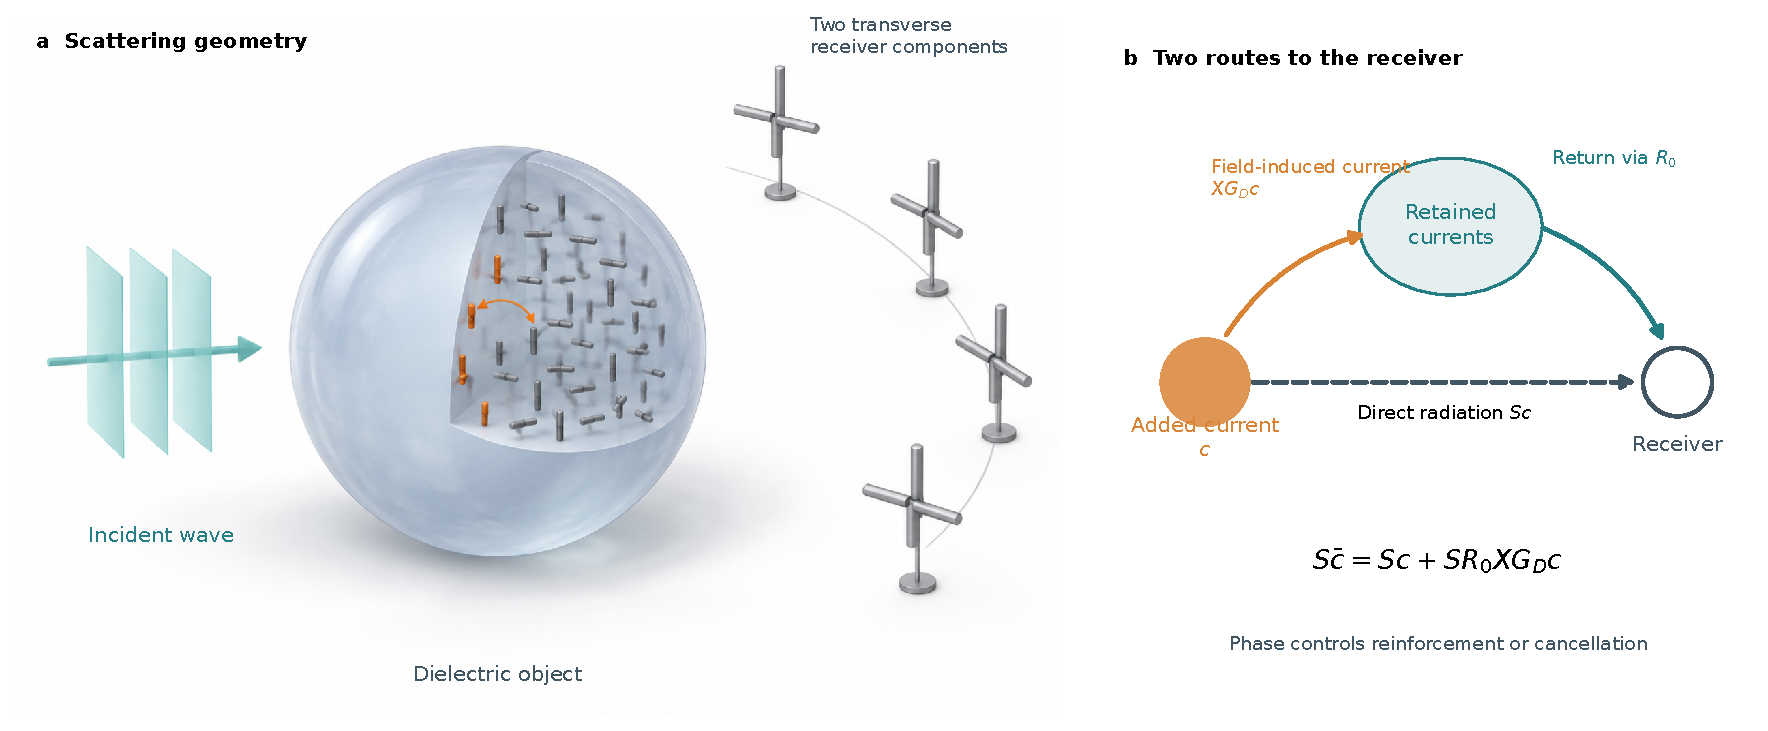
\includegraphics[width=.95\textwidth]{figures/physical_feedback.pdf}
\caption{Material excitation, internal feedback, and reception in a finite dielectric object. The direct radiation of an added current is only one route to the receiver; the retained currents can carry an additional response. The drawing is a conceptual geometry, not a computed field distribution.}
\end{figure*}
\section{Electromagnetic Entry, Feedback, and Observation}

\subsection{Physical tangent and frozen inverse problem}

Consider isotropic, nonmagnetic dielectric contrast \(\chi\) with a fixed acquisition geometry. For illumination \(p\), the contrast-source formulation is

\[
\begin{aligned}
j_p&=X(e_p^{\rm inc}+G_Dj_p),&
L&=I-XG_D,\\
L\,\delta j_p&=B_ps,&
B_ps&=DX[Q_Ts]e_p^{\rm tot}.
\end{aligned}\tag{1}
\]

Here \(G_D\) is the internal vector Green operator; \(X\) is the material response; \(e_p^{\rm tot}\) is the current total field; and \(Q_T\) expands a real material coordinate vector \(s\in\mathbb R^d\), including both parts of complex contrast. Thus \(d\) is the admissible real material dimension. Its realified expansion obeys \(Q_T^\top M_\chi Q_T=I\), with the volume-weighted material \(L^2\) metric \(M_\chi\). Current coordinates are also normalized to their declared discrete metric. With the receiver/scaling map \(S\),

\[
K_p=L^{-1}B_p,\qquad J_p=SK_p. \tag{2}
\]

The actual discrete-dipole approximation (DDA) uses contrast-dependent polarizability, rather than substituting \(X=\chi\) in its discrete equation. Its injection retains the polarizability derivative and the vector local field; Section 1 of the Supplement gives the exact implemented model. The operator identities use \(A=I-L\); \(A=XG_D\) expresses their contrast-source interpretation, and \(A=D_aG_{\rm off}\) is the implemented DDA counterpart.

Illuminations have separate currents and one shared material vector $s\in\mathbb R^d$. Each excitation $B_ps$ produces a current change $L^{-1}B_ps$ and measurement change $J_ps$. Stacking $[\operatorname{Re}(J_ps);\operatorname{Im}(J_ps)]$ over illuminations gives one real measurement vector. The normal equations are therefore real material-space equations, with $^*$ denoting the corresponding adjoint. The complex current-block identities lift through block-diagonal current operators and vertically stacked material injection (Section 1 of the Supplement).

At a frozen state, let \(r\) be predicted minus observed data, \(\Lambda\succ0\) the common regularization/damping curvature, and \(\ell\) its common linear prior term. Define the full quadratic

\[
\begin{aligned}
\Phi(s)&=\frac12\|r+Js\|^2\\
&\quad+\frac12s^*\Lambda s+\ell^*s\\
&=\frac12s^*Hs+h^*s+\frac12\|r\|^2,\\
H&=J^*J+\Lambda,& h&=J^*r+\ell.
\end{aligned}\tag{3}
\]

Thus \(s_*=-H^{-1}h\), and the squared \(H\)-energy step error is twice the full quadratic gap, providing an exact measure of local step quality. Subtracting the common constant \(\tfrac12\|r\|^2\) in stored relative objectives leaves all gaps and gains unchanged.

\subsection{Specified Galerkin enlargement}

Let \(V\) be an orthonormal current basis, \(C\) an orthonormal candidate bank with \(V^*C=0\), and assume \(V^*LV\) is invertible. The old Galerkin operators are

\[
\begin{aligned}
R_0&=V(V^*LV)^{-1}V^*,& K_0&=R_0B,\\
J_0&=SK_0,& H_0&=J_0^*J_0+\Lambda,\\
&&M_0&=H_0^{-1}.
\end{aligned}\tag{4}
\]

\(R_0\) solves a retained current equation; \(M_0\) solves a material normal equation. Put

\[
\begin{aligned}
\bar C&=(I-R_0L)C=C+R_0AC,& Y_C&=S\bar C,\\
N_C&=C^*(B-LK_0),& \Gamma_C&=C^*L\bar C.
\end{aligned}\tag{5}
\]

The symbol \(\Gamma_C\) denotes a current Schur matrix and is distinct from the receiver map \(S\). For \(A_{UV}=U^*AV\), \(D_V=I-A_{VV}\), \(B_V=V^*B\), and \(B_C=C^*B\), these factors become

\[
\begin{aligned}
\bar C&=C+VD_V^{-1}A_{VC},\\
Y_C&=SC+(SV)D_V^{-1}A_{VC},\\
N_C&=B_C+A_{CV}D_V^{-1}B_V,\\
\Gamma_C&=I-A_{CC}-A_{CV}D_V^{-1}A_{VC}.
\end{aligned} \tag{6}
\]

\textbf{Proposition 1 (feedback-dressed tangent factorization).} If \(\Gamma_C\) is invertible, the strictly Galerkin tangent in \([V,C]\) satisfies

\[
K_C-K_0=\bar C\Gamma_C^{-1}N_C,\qquad
\Delta J:=J_C-J_0=Y_C\Gamma_C^{-1}N_C. \tag{7}
\]

\textbf{Proof.} The enlarged coefficient matrix has blocks \(D_V,-A_{VC},-A_{CV},I-A_{CC}\). Eliminating its retained coordinates gives \(\Gamma_C\) and right-hand side \(N_C\). Back-substitution adds \(VD_V^{-1}A_{VC}\) to the raw candidate response \(C\), proving (6)--(7). It also gives \(V^*L\bar C=0\). \hfill\(\square\)

Equation (6) identifies three physical paths. First, an added current radiates directly through \(SC\), but also generates an internal field through \(G_D\), excites retained currents through \(X\), and radiates through \(SV\) after retained-space rescattering. Hence

\[
\boxed{\bar C=C+R_0XG_DC}
\]

in the contrast-source formulation. Second, material injection can enter the retained space through \(B_V\) before reaching the new coordinates through \(A_{CV}\). Third, \(A_{CV}D_V^{-1}A_{VC}\) is the added-to-retained-to-added loop, which enters the Schur inverse rather than a single-pass correction. The dressed current preserves the retained Galerkin equations through \(V^*L\bar C=0\), while generally losing Euclidean orthogonality to \(V\). For a receiver-dark candidate, the isolated direct branch \(SC\) is zero or near roundoff; internal scattering produces the nonzero dressed response \(S\bar C\).



\subsection{Weak relative feedback requires more than weak scattering}

If \(\|A_{VV}\|\le\eta<1\), a sufficient absolute bound is

\[
\|Y_C-SC\|\le
\frac{\|SV\|\,\|A_{VC}\|}{1-\eta}. \tag{8}
\]

To obtain a direction-uniform \emph{relative} bound on a candidate subspace, its direct radiation must also be bounded away from zero. If \(SC\) is injective there, then

\[
\frac{\|(Y_C-SC)a\|}{\|SCa\|}
\le\frac{\|SV\|\,\|A_{VC}\|}
{(1-\eta)\sigma_{\min}(SC)}
\quad(a\ne0). \tag{9}
\]

A singular \(SC\) requires restriction to a specified non-dark coefficient space. A sufficient Schur-invertibility condition is \(\|A_{CC}+A_{CV}D_V^{-1}A_{VC}\|<1\). These sufficient conditions separate weak absolute coupling from weak relative feedback. Small absolute feedback may dominate a nearly dark direct response; cross-space coupling and a large, possibly nonnormal retained resolvent provide additional amplification mechanisms. Their contributions must be resolved before attributing a large ratio to resonance.

\section{Paired Material Closure and Nonmonotone Curvature}

\subsection{The two-channel regularized step change}

For the material-space formulas below, the factors must be real-lifted together. Let $P$ be the number of illuminations, $\mathbf Y=I_P\otimes Y_C$, $\Gamma_{\rm blk}=I_P\otimes\Gamma_C$, and $\mathbf N=[N_{C,1}^\top,\ldots,N_{C,P}^\top]^\top$. Define $\mathcal R(F)=[\operatorname{Re}F,-\operatorname{Im}F;\operatorname{Im}F,\operatorname{Re}F]$ and $\widehat N=[\operatorname{Re}\mathbf N;\operatorname{Im}\mathbf N]$. Then $\widehat D=\mathcal R(\mathbf Y)\mathcal R(\Gamma_{\rm blk})^{-1}\widehat N$, up to the fixed stacking permutation. Throughout this material-space subsection, $Y_C,\Gamma_C,N_C$ denote these lifted factors, and $T_C=\Gamma_C^{-1}N_C$ is formed after lifting; their adjoints are real transposes. If $m$ is the complex receiver dimension per illumination and $r_c$ the added complex current rank, the lifted $Y_C$ has dimensions $2Pm\times2Pr_c$, and the lifted $N_C$ has dimensions $2Pr_c\times d$. This preserves the shared material variable and does not treat each complex current atom as a rank-one real material change.

Set \(T_C=\Gamma_C^{-1}N_C\). For the same \(B,r,\Lambda,\ell\), define

\[
\begin{aligned}
s_0&=-M_0(J_0^*r+\ell),\\
s_C&=-(J_C^*J_C+\Lambda)^{-1}(J_C^*r+\ell),\\
\mathcal E_0(C)&=\operatorname{Range}M_0[J_0^*Y_C,N_C^*].
\end{aligned}\tag{10}
\]

\textbf{Theorem 1 (paired step-change closure).} Under Proposition 1, with exact actions, positive regularization, and no nonzero signature removed,

\[
\begin{aligned}
s_C-s_0={}&-M_0J_0^*Y_C(T_Cs_C)\\
&-M_0N_C^*\Gamma_C^{-*}Y_C^*(r+J_Cs_C)
\in\mathcal E_0(C).
\end{aligned} \tag{11}
\]

\textbf{Proof.} Write \(\Delta H=J_C^*J_C-J_0^*J_0\) and \(\Delta h=\Delta J^*r\). Expanding \(J_C=J_0+Y_CT_C\) gives

\[
\Delta H=J_0^*Y_CT_C+T_C^*Y_C^*J_0+T_C^*Y_C^*Y_CT_C.
\]

Subtract the normal equations: \(H_0(s_C-s_0)=-\Delta Hs_C-\Delta h\). Collect the first observation term and the remaining \(T_C^*Y_C^*(r+J_Cs_C)\) term, and use \(T_C^*=N_C^*\Gamma_C^{-*}\). \hfill\(\square\)

The observation lift \(M_0J_0^*Y_C\) redistributes the update along old sensitivities when they couple to the added response. The injection lift \(M_0N_C^*\) pulls the updated data residual back through the new current excitation. Looking only at \(\Delta h\) retains the second channel and can miss the first channel's Hessian coupling.

The factors identify the available routes for material influence, while the coefficients in (11) determine how the present residual activates them. For example, when $r=0$ and $\ell=0$, both regularized steps vanish regardless of the derivative change. This separates structural coupling from its activation in a particular inverse step.

\subsection{Why one side is generally insufficient}

The exact illustration

\[
J_0=[1,0],\quad J_C=[1,1],\quad \Lambda=I,\quad r=1,\quad\ell=0
\]

gives \(s_0=(-1/2,0)^\top\), \(s_C=(-1/3,-1/3)^\top\), and \(s_C-s_0=(1/6,-1/3)^\top\). The observation lift is along the first material coordinate and the injection lift along the second. Neither alone contains the change. Although \(\Delta J=[0,1]\) has rank one,

\[
\Delta H=\begin{bmatrix}0&1\\1&1\end{bmatrix},\qquad\det\Delta H=-1. \tag{12}
\]

Both \(H_0=J_0^*J_0+\Lambda\) and \(H_C=J_C^*J_C+\Lambda\) remain positive definite under \(\Lambda\succ0\). The indefinite difference \(\Delta H\) describes redistribution of material curvature between these two well-posed regularized problems.

This algebraic illustration embeds in \(L=I\) Galerkin reduction: take $V=e_1$, $C=e_2$, $S=[1,1]$, and $B=I_2$. It isolates the least-squares effect: two-sided material coupling can occur even without scattering feedback. Feedback determines the electromagnetic factors; material least squares supplies the two-channel normal coupling.

\setcounter{equation}{12}
\section{Conditional Current Exchange and the Value of a Material Step}
\subsection{Changing a current model changes two material quantities}
A receiver-based space provides a reproducible starting approximation. At a fixed current budget, we can replace one of its directions while retaining the others. This asks a local design question: does the replacement improve the material step generated by the model? The test keeps the material state, illumination, physical tangent, residual, prior term and damping fixed.

Let the old and new current spaces be $[V,A]$ and $[V,C]$. When the common-core and Schur systems are invertible, their Jacobian difference is
\begin{equation}\label{eq:exchange-difference}
 D=Y_C\Gamma_C^{-1}N_C-Y_A\Gamma_A^{-1}N_A.
\end{equation}
These are two changes relative to the same retained core. If that core is singular, stable endpoints may still exist; then we compute the endpoints directly rather than using this elimination.

In the common real material coordinates, write $\mathsf I_U=J_U^TJ_U$ for the data curvature. A current change alters both data curvature and the constant gradient term:
\begin{equation}\label{eq:information-offset}
\begin{aligned}
 \Delta\mathsf I&=J_o^TD+D^TJ_o+D^TD,\\
 h_U&=J_U^Tr+\ell,\qquad \Delta h=D^Tr.
\end{aligned}
\end{equation}
Here the normal equation is $H_Us_U=-h_U$. The data curvature describes which material changes produce a measured response. The constant term describes how those responses align with the present residual. Both determine the actual endpoint step difference:
\begin{equation}\label{eq:exchange-step}
 d=s_n-s_o=-H_n^{-1}(\Delta h+\Delta\mathsf I s_o).
\end{equation}
The formula follows by subtracting the two normal equations. It applies to the fixed unconstrained quadratic; changing an active constraint set requires its own optimality equations.

Information magnitude alone cannot select this step. Even the scalar models $J_o=1$ and $J_n=-1$ have identical data curvature but opposite steps for $r=1$, $\ell=0$ and $\Lambda=1$. More generally, $\Delta\mathsf I$ can be indefinite: changing the approximation to existing data includes interference terms, unlike adding independent measurements.

\subsection{Evaluate the displacement actually produced}
For the unchanged full quadratic, a proposed displacement $d$ from $x$ has signed gain. In current exchange, $x=s_o$ is the old endpoint material step:
\begin{equation}\label{eq:exchange-gain}
 Q=\Phi_F(x)-\Phi_F(x+d)=-g_F(x)^Td-\tfrac12d^TH_Fd.
\end{equation}
Positive gain means a better approximation to this frozen full-model material update. It does not by itself determine material truth error. The latter also contains a cross term with the unknown material error, and nonlinear reconstruction additionally requires feasible updates and step acceptance.

The scalar gain can be checked without a new full adjoint. Cache $u=r+J_Fx$ and compute $z=J_Fd$. Then
\begin{equation}\label{eq:directional-exchange-gain}
 Q=-u^Tz-(\ell+\Lambda x)^Td-\tfrac12(\|z\|^2+d^T\Lambda d).
\end{equation}
For complex data the first product is $\operatorname{Re}\langle u,z\rangle$. Each full directional action still pays for every illumination. After an accepted move, the endpoint and conditional candidate scores change; the cached output updates as $J_Fx\leftarrow J_Fx+z$.

If validated output-error bounds $e_u,e_z$ are available, the computed gain has error at most
\begin{equation}\label{eq:exchange-gain-bound}
 \epsilon_Q=e_u\|\widehat z\|+(\|\widehat u\|+\|\widehat z\|)e_z+e_ue_z+\tfrac12 e_z^2.
\end{equation}
A positive lower bound can justify acceptance. A local stopping certificate instead requires an upper bound below tolerance for every feasible move in the declared neighborhood. A shortlist with no accepted move does not establish that condition. The computations below use double-precision full directional checks; a rigorous output bound is unavailable, so their numerical acceptance and stopping status are reported separately.

\subsection{Information diagnostics and their scope}
We normalize data curvature with a fixed positive material scale $P_0$, kept separate from numerical Levenberg--Marquardt damping. For eigenvalues $\nu_i$ of $P_0^{-1/2}\mathsf I_UP_0^{-1/2}$, we record
\begin{equation}
 d_{\rm eff}=
 \sum_i\frac{\nu_i}{1+\nu_i},\qquad
 \mathcal D=\tfrac12\sum_i\log(1+\nu_i).
\end{equation}
These quantities summarize the response claimed by a model. We also measure its curvature discrepancy from the full reference. Greater $\mathcal D$ need not mean greater fidelity, and neither scalar retains the residual-dependent term in~\eqref{eq:information-offset}. The present data normalization is a prescribed numerical scale, not an independently calibrated noise covariance; no mutual-information interpretation is needed.

Small Gaussian material spaces permit complete reference diagnostics. For the larger voxel spaces, all endpoints use the same sixteen material probe directions; those information measures describe that projection only. Information diagnostics, full-reference steps and material truth remain evaluation data, separate from the reduced-reference scores used to propose exchanges.

\section{Receiver-Centered Conditional Exchange}
\subsection{Proposal, finite check, and recomputation}
For each state, start with the first $k$ receiver singular directions, with $k=4,8,16$ complex current columns shared by all illuminations. Subsequent exchanges can replace these directions; the preserved quantity is current rank, not every original receiver column. The admissible real material coordinates, forward residual, material injection, prior, and damping are unchanged. An auxiliary common embedding caches the projected current, receiver, and injection operators. Its dimension is not the retained current dimension: each evaluated Galerkin endpoint still has exactly $k$ independent columns. This is a comparison at equal representation dimension. Anchor acquisition, the dictionary and directional checks are additional information and computation paid by the exchange policy, and are recorded separately.

The frozen proposal rule uses the existing current dictionary and a family-balanced pool of 12 incoming atoms. Its six sources are receiver modes, internal-propagation modes, Fourier modes, anchor primal/dual responses, anchor current-equation residuals, and fixed random currents. Cycling through this fixed source order selects two available atoms per source, excluding already selected atoms. A 64-column reduced anchor supplies an independent approximation to the full quadratic for ranking. Removing one retained atom and adding one incoming atom defines a concrete replacement. We solve its endpoint material problem and rank the actual displacement using the anchor finite gain. All conditional factors, including the complete Schur coupling, are recomputed after an accepted action. Singular common cores use stable direct endpoint calculations; endpoints failing the frozen current-stability or normal-equation-residual criteria are rejected. Both relative cutoffs are $10^{-10}$; a small normal residual and a well-conditioned current block are separate requirements.

Only the two highest-ranked feasible finalists receive full directional checks. The current output $J_Fx$ is cached and a finalist requires $J_Fd$. Each direction costs one current right-hand side per illumination. Among the checked finalists, the largest gain above the online numerical tolerance is accepted. Otherwise the state remains unchanged and the algorithm abstains within its tested pool. The procedure terminates after three accepted replacements or an abstention. Untested incoming atoms can contain useful actions, so this stopping rule does not establish full-dictionary local optimality.

\subsection{An online numerical significance threshold}
All proposal and acceptance inputs are available without the full optimal material step. For FP64 arrays define
\begin{equation}\label{eq:online-scale}
\begin{split}
S_Q={}&\sum_i|u_i||z_i|+\sum_j|(\ell+\Lambda x)_j||d_j|\\
&+\tfrac12\|z\|^2+\tfrac12\lambda\|d\|^2+\|r\|^2+\|u\|^2\\
&+|\ell^Tx|+\lambda\|x\|^2,
\end{split}
\end{equation}
where the implemented regularization is $\Lambda=\lambda I$. With $m_R$ real data entries, $d_R$ real material entries, machine precision $\epsilon_{64}$, and $n=m_R+3d_R+16$, use
\begin{equation}\label{eq:online-tolerance}
\tau_{\rm online}=32\,\mathrm{tiny}_{64}
+32\frac{n\epsilon_{64}}{1-n\epsilon_{64}}S_Q.
\end{equation}
Here $\mathrm{tiny}_{64}$ is the smallest positive normal FP64 number, as returned by the implemented floating-point type. The factor 32 and summation scale were fixed analytically before validation. The initial-output terms retain the numerical scale when a proposed displacement is extremely small. This tolerance assesses floating-point significance in the reported gain; it is not a bound on Maxwell discretization or current-solve output error. The present experiments therefore use \emph{high-fidelity numerical verification}. A deterministic acceptance certificate would additionally require the valid output-error radii stated in the preceding section.

The earlier evaluation-derived floor is excluded from the controller. Physical replay of all 36 original cells verifies this change: all 75 accepted replacements, final spaces, material steps, and directional outputs are unchanged. The replayed final and receiver gaps each agree exactly with their pre-replay values. Full optimal steps are loaded only after all online endpoints for a state have been saved, for evaluation.

\subsection{What is evaluated}
The primary metric is the frozen full-GN quadratic gap
\begin{equation}\label{eq:gn-gap}
R_{\rm GN}(U)=\Phi_F(s_U)-\Phi_F(s_*)
=\tfrac12\|s_U-s_*\|_{H_F}^{2}.
\end{equation}
The identity in (\ref{eq:gn-gap}) uses the exact optimizer. A numerically converged reference $\tilde s_*$ retains the term $g_F(\tilde s_*)^T(s_U-\tilde s_*)$ when its quadratic gap is evaluated; the true reference residual and evaluation-only floor are stored separately. The full optimizer is an offline reference. Each object is summarized by the sum of its eligible state--budget gaps divided by the corresponding receiver sum. Absolute gaps and normalized $H_F$ step errors accompany ratios, particularly when the receiver gap is small. Independent aggregation and bootstrap resampling use objects; multiple states and budgets of one object are correlated measurements.

For nonlinear transfer, both policies use the same full forward model, physical material parameterization, constraints, damping, prior, and line search. Only the tangent-current policy changes. The finite frozen gain applies to its unprojected displacement. A projected or backtracked nonlinear step is subsequently judged by the common full nonlinear objective.

\section{Physical Evidence: Coupling Is Not Yet Utility}
These controlled examples isolate why direct radiation and information summaries can miss material-update consequences. They establish possible mechanisms in vector Maxwell discretizations. The subsequent exchange validation measures utility directly; it does not attribute every accepted gain to a dark-current path or to one feedback channel.
\subsection{A directly dark current can return through scattering}
The first test isolates the receiver path. In controlled $5^3$, $6^3$, and $7^3$ vector-Maxwell grids, a two-column candidate is constructed in the numerical null space of the direct receiver map. Its direct output norm is below $1.7\times10^{-16}$. The dressed outputs $S\bar C$ have norms 0.0672, 0.0720, and 0.0888, respectively. The corresponding specified enlargement changes the material derivative by 3.56\%, 3.98\%, and 5.22\%. The candidate becomes observable through retained-space scattering, despite negligible isolated radiation. This is a mechanism witness, rather than a claim that all weak receiver modes are useful.

\begin{figure}[t]\centering
\includegraphics[width=\linewidth]{figures/path_depth_dark.pdf}
\caption{Directly dark directions return through retained scattering in the controlled Maxwell example. The direct branch alone misses a measurable derivative change. Grid refinement here tests this mechanism; independent continuum validation of every material direction is not implied.}
\end{figure}

\subsection{More apparent information can produce a worse step}
Data curvature $\mathsf I_U=J_U^TJ_U$ describes the material response claimed by a reduced model. Relative to a positive scale $P_0$, let $\nu_i$ be the eigenvalues of $P_0^{-1/2}\mathsf I_UP_0^{-1/2}$. Two familiar summaries are
\begin{equation}
\mathcal D(U)=\tfrac12\sum_i\log(1+\nu_i),\qquad
d_{\rm eff}(U)=\sum_i\frac{\nu_i}{1+\nu_i}.
\end{equation}
We use $P_0=10^{-5}I$. These summaries quantify information magnitude relative to that declared scale; measured noise-covariance calibration is not assumed. Information fidelity is a different question: how closely does this curvature approximate the full curvature? We use the offline diagnostic $e_I(U)=\|(\mathsf I_F+P_0)^{-1/2}(\mathsf I_U-\mathsf I_F)(\mathsf I_F+P_0)^{-1/2}\|_2$, where $\mathsf I_F=J_F^TJ_F$; a smaller value means closer normalized curvature.

A saved near-contact Maxwell replacement at $k=4$ increases $\mathcal D$ by 6.3127 and $d_{\rm eff}$ by 1.8613. Its normalized curvature-fidelity diagnostic improves slightly, yet its full finite gain is $-5.5754\times10^{-5}$. The replacement worsens the full material step. The displacement equation explains why: $\Delta h$ and $\Delta\mathsf I s_o$ jointly enter the step. Neither information magnitude nor one curvature-fidelity scalar determines their residual-dependent effect. This witness does not isolate the offset as the sole cause.

\subsection{Relevance can depend on another added direction}
From the same rank-14 Maxwell core, two single additions give
\[
Q_A=-3.2391\times10^{-8},\qquad Q_B=-5.8389\times10^{-8},
\]
whereas their joint rank-16 addition gives $Q_{AB}=+3.4787\times10^{-7}$. Five of 540 predeclared pair tests have this singleton-negative, pair-positive pattern. This finite set demonstrates conditional, non-additive utility. It is neither a probability estimate over Maxwell modes nor a same-rank exchange trap. The fixed one-out/one-in method is retained; the pair witness explains a design boundary, rather than motivating an added search rule.

\begin{figure*}[t]\centering
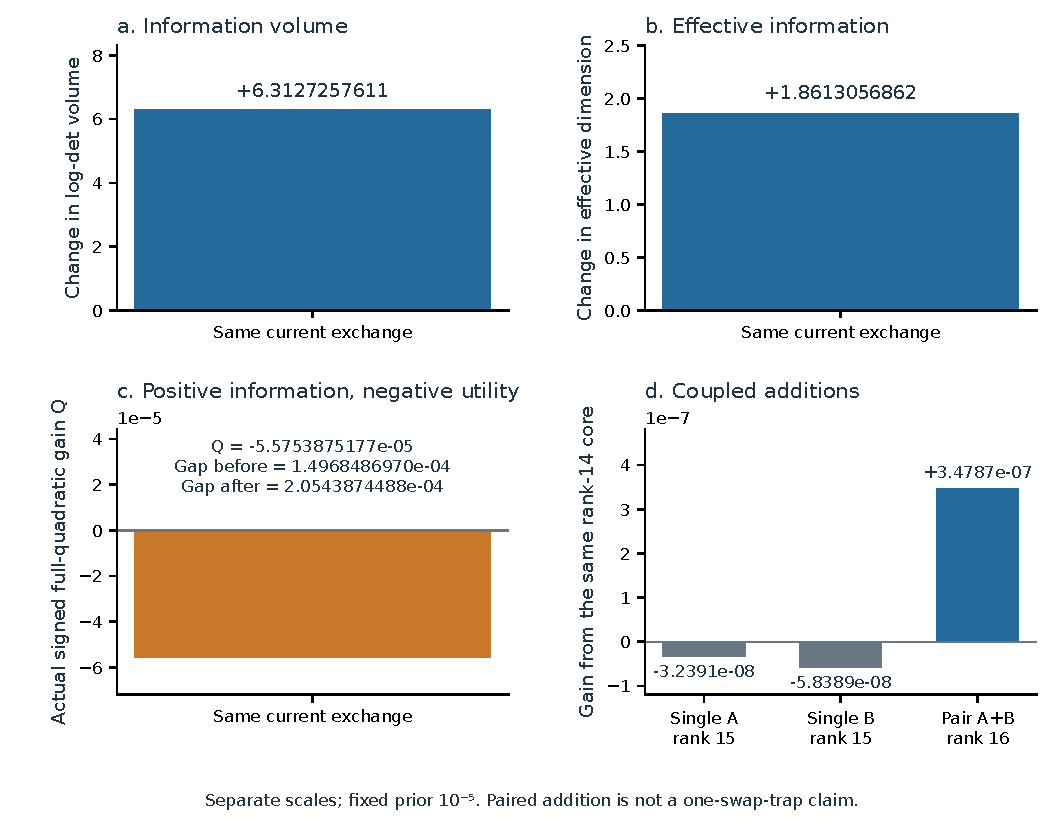
\includegraphics[width=.9\textwidth]{figures/information_and_pair_witness.pdf}
\caption{Two distinct witnesses. Increased information magnitude and slightly improved curvature fidelity coexist with negative material gain. Separately, two individually unfavorable additions become favorable when combined. The quantities have different units and are not combined into a universal score.}
\end{figure*}

\subsection{The cost of the actual finite displacement changes ordering}
A controlled $2\times2$ diagnostic separates the displacement from its evaluation. For common candidates, $v$ uses the old Hessian's first-order displacement and $d=s_n-s_o$ is the actual endpoint difference. Each is ranked by either its linear term or its full quadratic expression, and the selected replacement is evaluated using its actual $d$.

When a top-one action is mandatory and no-op is deliberately removed, the linear score $-g_F^Td$ selects a negative-gain replacement in 29 of 36 cells. Including $-\tfrac12d^TH_Fd$ reduces this count to 1 of 36. Finite-displacement curvature cost materially changes candidate ordering in these cases. The counts describe the controlled diagnostic; deployed conditional exchange separately rejects unfavorable checked actions. An older finite/first-order risk ratio also changed displacement construction and terminal search, and is not used to attribute an improvement to the curvature term alone.

\section{Locked Three-Dimensional Validation}
\subsection{Common physical problem and comparison}
The experiments use the same vector-Maxwell DDA state and derivative operators throughout; general DDA background is given in~\cite{r11}. Six transverse plane-wave illuminations and 64 dual-polarization receivers sample the scattered field. The inverse grid has $12^3$ cells in a box of side 1.5, with $k_0=2$; truth data use a $14^3$ grid. Both grids use the same DDA family. The material coordinates are volume-orthonormal Gaussian or voxel tangents, with the true polarizability derivative retained. The full forward residual and injection are common to both policies; only the tangent-current space changes. Current ranks $k=4,8,16$ are actual shared complex columns, distinct from the real material dimension. The Supplement provides the implemented dyadic, acquisition, gauges, and hash-locked protocol.

We compare the unchanged receiver backbone with the frozen verified-exchange rule. Each object contributes the initial linearization, saved iteration index 3, and last saved linearization. A complete object therefore has nine state--rank cells. We aggregate absolute full-GN gaps within an object before dividing by its receiver total. The independent aggregation unit is the object, not a state or rank. A 10,000-draw object bootstrap uses the predeclared seed 20261002.

\subsection{Original objects and additional-object validation}
The original smooth Gaussian, near-contact Gaussian, layered voxel, and asymmetric voxel objects give 35 improved cells and one equal cell out of 36. Their object-summed gap ratios are 0.1904,0.6538,0.2776, and 0.4181; the median 0.3478 represents a 65.2\% reduction. The physical threshold replay preserves all these results.

Before additional results, we locked the rule, thresholds, seeds, and all eleven remaining compatible objects. Ten objects provide complete nine-cell coverage and all ten improve. Their median object-summed ratio is 0.4928, a 50.7\% reduction; the interquartile range is [0.3314,0.5588] and the object-bootstrap 95\% interval for the median is [0.3133,0.5647]. The remaining asymmetric voxel object completes six early/middle cells, with ratio 0.4925. Its late receiver endpoint fails the frozen normal-residual check at the first budget; the two subsequent budgets are not run. All three unavailable cells remain in the 99-cell denominator.

Among the 96 audited additional-object cells, 95 improve, one is equal within the evaluation floor, and none worsen. Absolute receiver gaps span $2.74\times10^{-7}$--$3.09\times10^{-3}$; exchange gaps span $8.73\times10^{-8}$--$8.36\times10^{-4}$. The smallest receiver denominator exceeds its evaluation floor by $6.31\times10^9$, and the maximum full-reference true normal residual is $9.55\times10^{-12}$. The improvement is resolved in the stored absolute quantities, rather than created by dividing two floor-level risks. Figure~\ref{fig:locked-primary} reports both ratios and absolute gaps.

\begin{figure*}[t]\centering
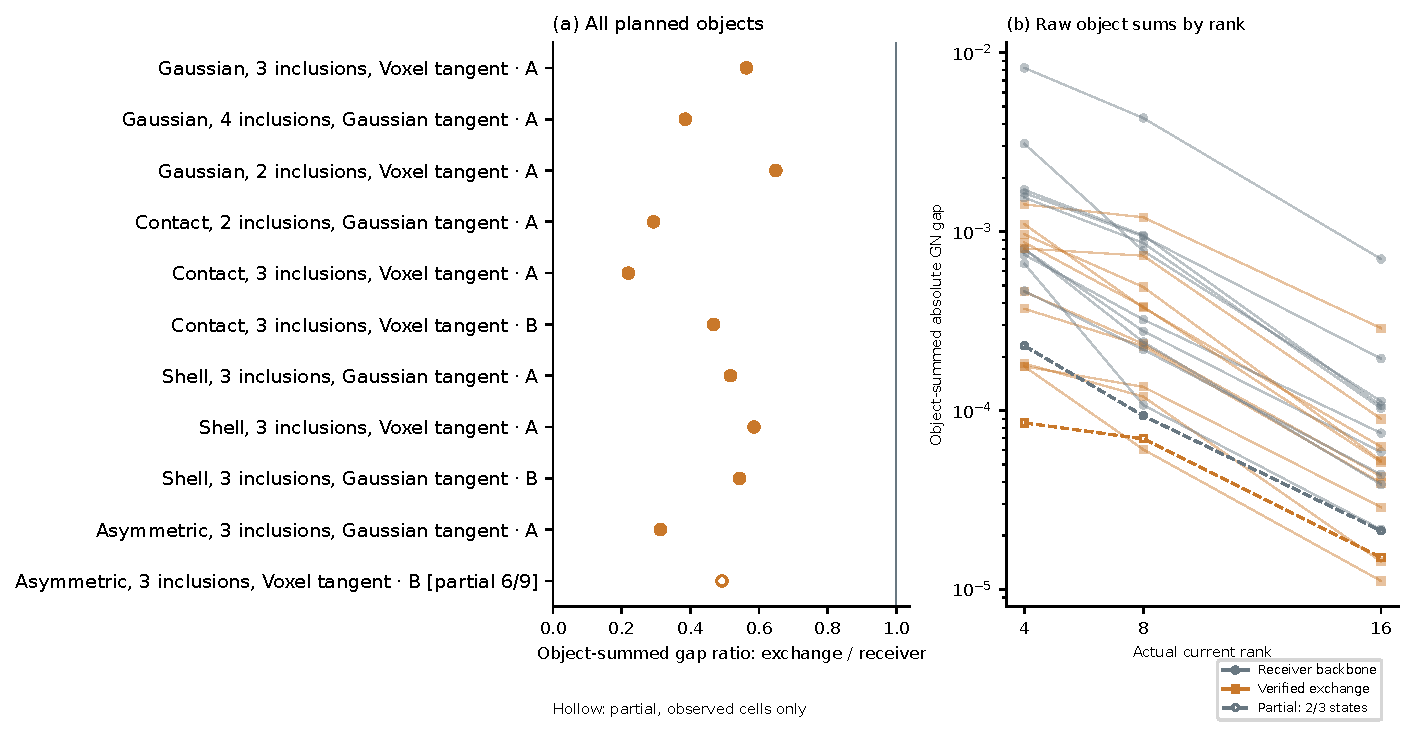
\includegraphics[width=.92\textwidth]{figures/closure_validation_v2/Figure1_primary_overview.pdf}
\caption{Frozen-rule validation on all planned additional objects. Left: object-summed full-GN gap ratios; filled markers are ten complete objects, while the hollow marker uses six of nine cells from the remaining object. Right: paired absolute gap sums by current rank; dashed curves retain that object's two available states. Geometry labels distinguish smooth profiles, contact structures, shells, and asymmetric structures; the complete representation mapping is in the Supplement. These quantities measure frozen material-step fidelity.}\label{fig:locked-primary}
\end{figure*}

These additional objects were historically studied in a broader current-ranking investigation. Inspected records show no object-specific use in historical exchange-teacher or pilot-network development, but complete blind independence cannot be established from their historical exposure. We therefore describe this test as locked-rule validation on additional previously studied Maxwell objects. The bootstrap summarizes this fixed object set; it is not a distribution-free generalization guarantee.

\subsection{Noisy residuals}
Four objects were preselected by geometry and representation: smooth voxel, near-contact Gaussian, shell Gaussian, and asymmetric voxel. Their middle-state physics is fixed while 1\% and 3\% relative complex noise changes the residual, with three independent realizations at each level. Every noisy residual receives its own offline full-GN reference after online selection. All 72 planned cells are audited: 71 improve and one abstains with an unchanged gap. The median object-summed ratios are 0.3307 at 1\% and 0.4026 at 3\% (Table~\ref{tab:noise}).

The controller verifies 408 finalists and rejects 98 below the numerical threshold; 172 exchanges are accepted. Verification costs 2448 current right-hand sides for $Jd$, including rejected finalists. Selected directions change with the residual, so this evidence concerns retained update utility rather than invariance of selected modes. The limited four-object, middle-state test supports the effect at these two noise levels.

\begin{table}[t]\centering\caption{Noise: ratio of object-summed full-GN gaps. Each entry sums three realizations and three current ranks.}\label{tab:noise}
\begin{tabular}{lrr}\toprule
Geometry / material tangent&1\%&3\%\\\midrule
Smooth / voxel&0.3255&0.4384\\
Near-contact / Gaussian&0.0996&0.1873\\
Shell / Gaussian&0.3358&0.3667\\
Asymmetric / voxel&0.3687&0.5330\\\midrule
Object median&0.3307&0.4026\\\bottomrule
\end{tabular}
\end{table}

\subsection{Ranking, candidate coverage, and exchange paths}
An offline diagnostic enumerates every feasible initial one-out/one-in replacement in the fixed 154-atom dictionary, then follows at most three full-score greedy exchanges. Its labels are acquired after the online decisions and never change them. The 96 available cells are complete; the three cells excluded by the earlier endpoint failure remain unrun.

Across the ten complete additional objects, the reduced anchor's full-dictionary top choice captures 97.30--99.99\% of the summed positive initial-exchange opportunity (median 99.54\%). Restricting acquisition to the frozen 12-atom incoming pool captures 49.12--95.31\% (median 72.95\%). Thus candidate acquisition, rather than reduced ranking alone, is the larger limitation in this test. These are positive-gain-weighted initial-neighborhood captures, not the improvement fraction of the deployed multistep method. The separate bounded greedy path reaches a smaller final gap in 90 of 96 cells, the online path is smaller in five, and one agrees within the evaluation floor. A greedy path is a local diagnostic, not a global optimum; its difference from deployment combines coverage, ranking, and path interactions.


\subsection{Constrained nonlinear transfer}
Four objects were fixed by geometry and material representation before validation. At $k=8$, both policies use the same initialization, prior, damping schedule, material constraints and full-objective Armijo line search. Only the tangent-current policy changes. Three paired trajectories complete all 18 updates. Table~\ref{tab:nonlinear} reports their complete-volume material errors and held-out data errors.

\begin{table*}[t]\centering
\caption{Constrained nonlinear transfer: receiver $\rightarrow$ verified exchange. Material errors are relative full-volume norms. Child wall includes each policy's own physical setup, acquisition, all outer work and terminal evaluation. Each trajectory is timed once.}\label{tab:nonlinear}
\begin{tabular}{lrrrr}\toprule
Geometry / material tangent&Complex material&Real material&Imaginary material&Held-out data\\\midrule
Smooth / voxel&$0.3027\to0.2699$&$0.2811\to0.2516$&$0.7439\to0.6506$&$0.006637\to0.002836$\\
Near-contact / Gaussian&$0.6722\to0.6707$&$0.6810\to0.6835$&$0.4439\to0.2859$&$0.010521\to0.007080$\\
Shell / Gaussian&$0.6096\to0.5660$&$0.6081\to0.5651$&$0.6976\to0.6219$&$0.014190\to0.012179$\\\midrule
Geometry / material tangent&\multicolumn{2}{c}{Child wall (s)}&Wall ratio&Total full tangent RHS\\
Smooth / voxel&\multicolumn{2}{c}{$216.5\to579.9$}&2.68&$0\to708$\\
Near-contact / Gaussian&\multicolumn{2}{c}{$407.7\to710.5$}&1.74&$0\to744$\\
Shell / Gaussian&\multicolumn{2}{c}{$405.9\to592.3$}&1.46&$0\to744$\\\bottomrule
\end{tabular}
\end{table*}

Complex-material error decreases by 10.8\%, 0.22\%, and 7.16\%, respectively, and held-out errors decrease in all three pairs. The near-contact real-part error increases slightly, so improved data fit does not imply uniform component recovery. The fourth object's exchange trajectory retains 17 completed updates. Before update 18, its receiver-derived starting endpoint fails the fixed normal-residual check, stopping that exchange trajectory. The separate receiver-only baseline job is not run after the queue stops. The four-object denominator and both unavailable final endpoints remain explicit.

These trajectories support a limited reconstruction consequence of the frozen rule. They also separate fidelity from efficiency: the complete child-wall ratios range from 1.46 to 2.68. Extra tangent actions purchase checked material changes; faster imaging is not established.

\begin{figure*}[t]\centering
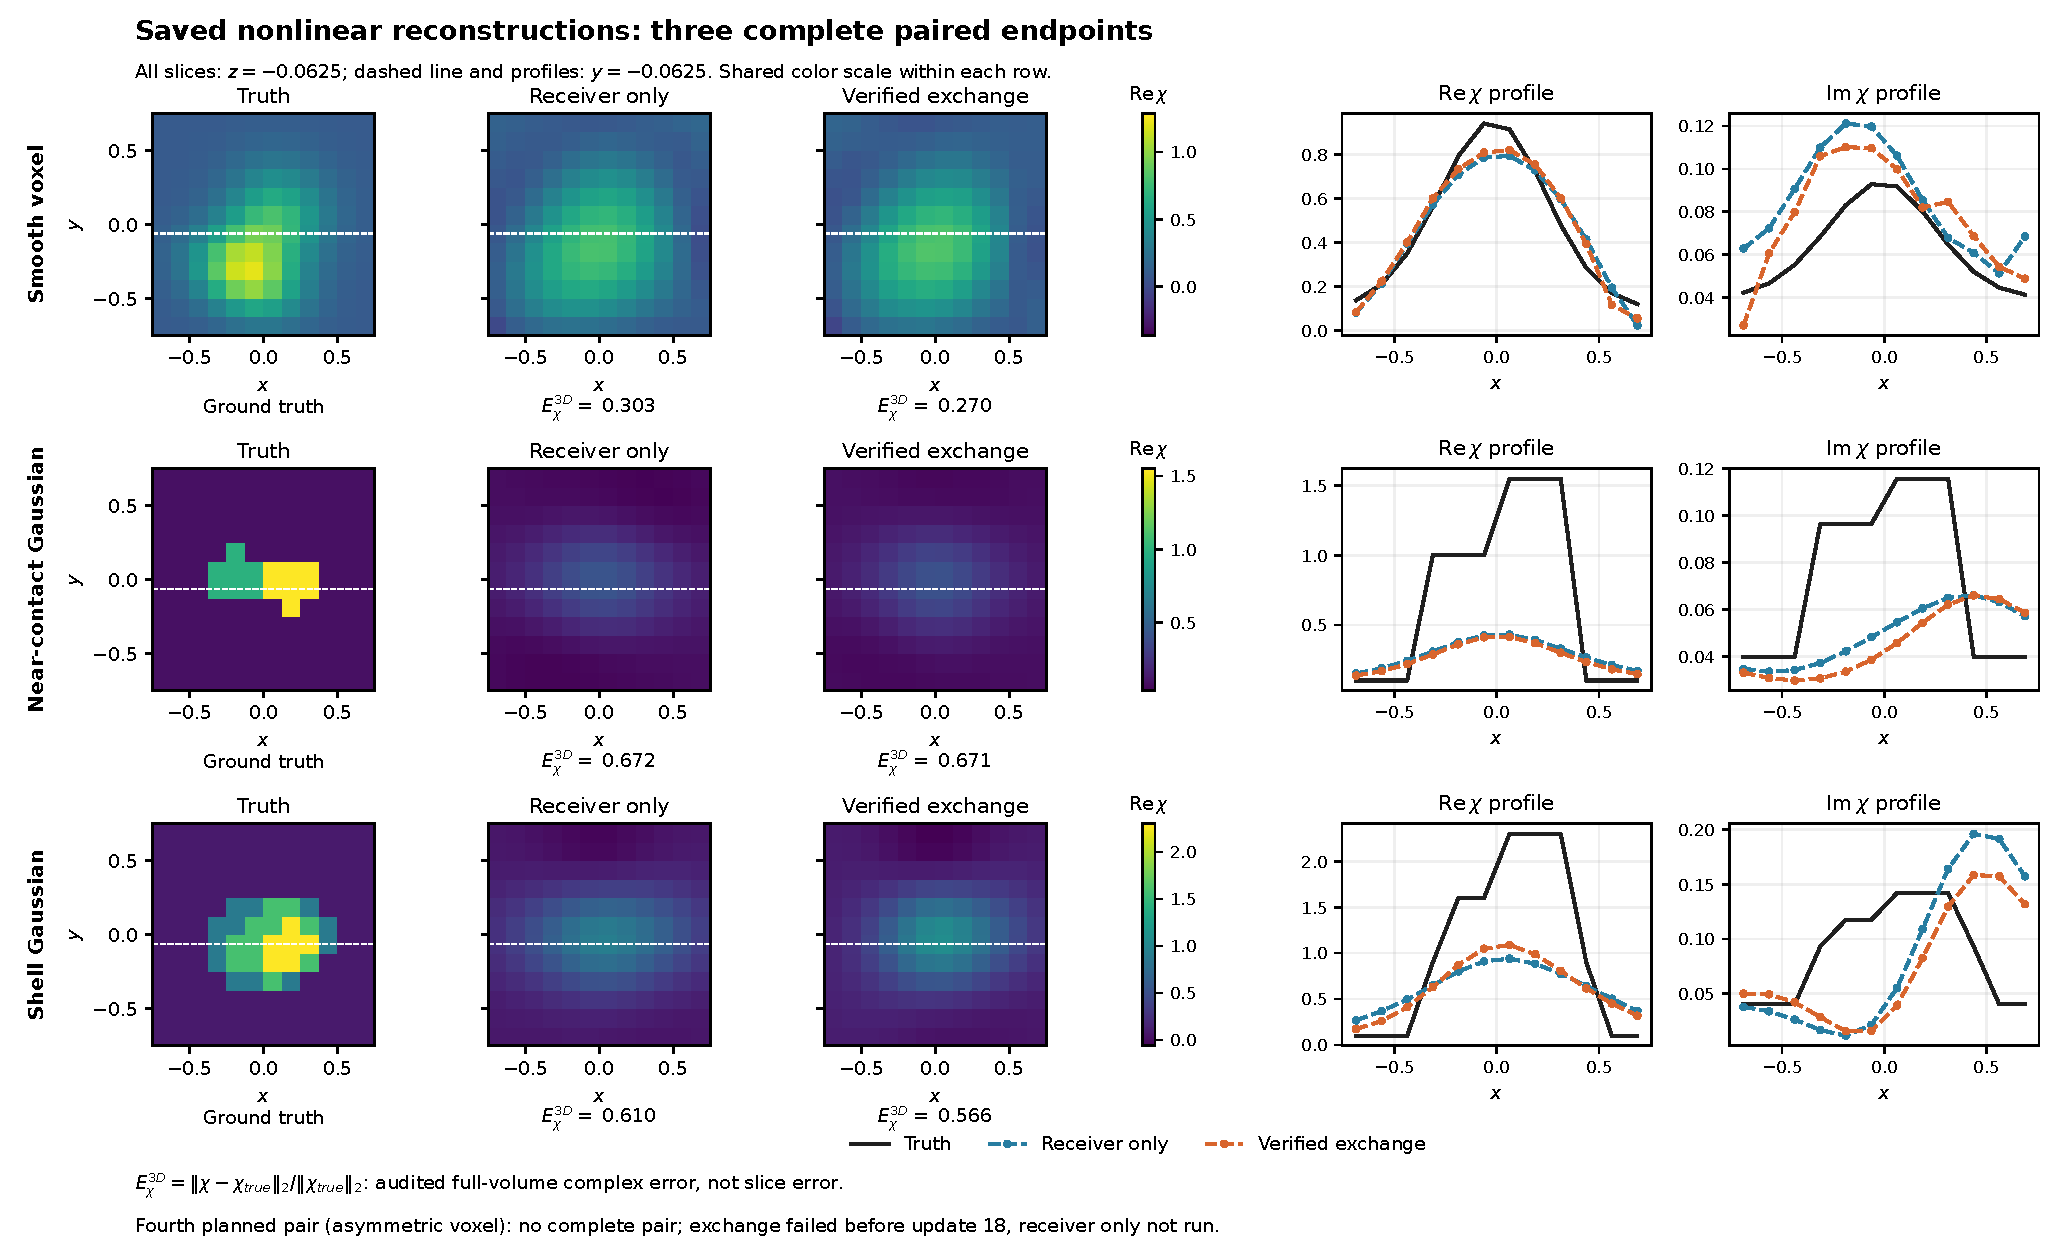
\includegraphics[width=.92\textwidth]{figures/nonlinear_closure_v1/nonlinear_reconstructions.pdf}
\caption{Complete nonlinear pairs at current rank eight. The real-material slices use the same central inverse-grid plane and a common color scale within each row; line profiles compare both real and imaginary contrast. These images accompany complete-volume errors in Table~\ref{tab:nonlinear}. The contact and shell peaks remain blurred despite improved data fit. The asymmetric voxel pair has no completed paired endpoint and is retained separately in the failure record.}\label{fig:nonlinear-slices}
\end{figure*}


\subsection{The added price of a current-space decision}
Exchange pays for the richer anchor, candidate acquisition, endpoint proposals and full directional checks beyond the unchanged receiver endpoint. The frozen workflow shares projected operators; a separate cold receiver-only build was not timed, so its warm selection wall is not an end-to-end baseline. The independently initialized nonlinear trajectories provide the all-in comparison: exchange takes 2.68, 1.74 and 1.46 times receiver-only child wall in the three complete pairs. The design purchases material-step fidelity with additional physics work.

Full campaign accounting, including historical carry, failed launches, verification, references and offline full-dictionary diagnostics, closes at 19,962.060~s (5.545~h). This is an execution-accounting total, rather than a per-solve runtime. The Supplement distinguishes additive occupation from nested stage and action counts; no acceleration follows from either a warm selection time or one reduced class of right-hand sides.



\section{Design Implications and Limits}
The mechanism yields a useful sequence of questions. Can a material perturbation enter the proposed current direction? Can that direction return to the receiver after retained-space scattering? Does the resulting finite material displacement reduce the present full quadratic? These questions concern different operators and cannot be replaced by one unconditional current ranking.

Conditional exchange starts from a stable receiver-derived space and changes its directions through a small number of checked replacements. No-op avoids accepting an unfavorable checked action; the substantive result is the measured decrease in absolute and object-summed full-GN gaps. A fixed current dimension controls representation size, not construction or verification cost. Each improvement purchases additional physics actions, whose setup, proposal, rejection, and offline evaluation costs remain visible.

The incoming pool restricts which opportunities can be tested. Full-dictionary reduced ranking can be accurate while the 12-atom pool omits a valuable direction, and successive exchanges can enter different local neighborhoods. Candidate coverage, scoring error, and path interactions are reported separately. Improving candidate acquisition is future work; the present method and validation do not add a learned proposer.

The GN metric measures fidelity to a specified regularized local update. It is not truth error, and a full GN step can itself be a poor estimator under limited data or inappropriate regularization. Constraints and nonlinear acceptance act on a different executed displacement. Their common line search is essential to interpreting transfer to a final material estimate. Likewise, an FP64 numerical significance threshold does not establish a deterministic output-error radius or a discretization-independent safety guarantee.

The Maxwell contribution is the explicit entry--feedback--return path of a specified current-space modification and its residual-dependent material utility. TSOM already incorporates internal propagation, and generic goal-oriented reduction already uses task information. The physical factorization, concrete dark-current and interference witnesses, and fixed-dimension exchange evidence provide the electromagnetic design content. Primary-source gaps preclude historical priority claims.

\section{Conclusion}
A receiver current space should be modified according to the material step that a specified replacement actually produces. Eliminating retained currents exposes the feedback-dressed observation and material injection factors, while the normal equations expose both curvature change and residual pullback. Their finite signed gain supplies a direct test on a common material quadratic. At unchanged endpoint current rank, the locked rule reduces the median summed gap by 50.7\% across ten complete additional Maxwell objects. The effect persists in the bounded noisy-residual tests and has a limited reconstruction consequence in three completed constrained pairs. The resulting design principle is operational: trace a current replacement through material excitation and receiver return, then check the finite material displacement before committing to the modified space.

\IEEEtriggeratref{9}
\begin{thebibliography}{99}
\bibitem{r1} Y. Zhong and X. Chen, ``An FFT Twofold Subspace-Based Optimization Method for Solving Electromagnetic Inverse Scattering Problems,'' \emph{IEEE Trans. Antennas Propag.}, vol. 59, no. 3, pp. 914--927, 2011, doi: 10.1109/TAP.2010.2103027.
\bibitem{r2} X. Ye and X. Chen, ``Subspace-Based Distorted-Born Iterative Method for Solving Inverse Scattering Problems,'' \emph{IEEE Trans. Antennas Propag.}, vol. 65, no. 12, pp. 7224--7232, 2017, doi: 10.1109/TAP.2017.2766658.
\bibitem{r3} X. Chen, \emph{Computational Methods for Electromagnetic Inverse Scattering}. Wiley--IEEE Press, 2018, Secs. 6.3.1 and 6.4.2.
\bibitem{r4} E. de Sturler, S. Gugercin, M. Kilmer, S. Chaturantabut, C. Beattie, and M. O'Connell, ``Nonlinear Parametric Inversion Using Interpolatory Model Reduction,'' \emph{SIAM J. Sci. Comput.}, vol. 37, no. 3, pp. B495--B517, 2015, doi: 10.1137/130946320. Author preprint: arXiv:1311.0922.
\bibitem{r5} M. Kartmann, T. Keil, M. Ohlberger, S. Volkwein, and B. Kaltenbacher, ``Adaptive Reduced Basis Trust Region Methods for Parameter Identification Problems,'' 2024, doi: 10.1007/s44207-024-00002-z. Author full text: arXiv:2309.07627v3.
\bibitem{r6} T. Bui-Thanh, K. Willcox, O. Ghattas, and B. van Bloemen Waanders, ``Goal-Oriented, Model-Constrained Optimization for Reduction of Large-Scale Systems,'' \emph{J. Comput. Phys.}, vol. 224, no. 2, pp. 880--896, 2007, doi: 10.1016/j.jcp.2006.10.026.
\bibitem{r8} A. Gaul, M. H. Gutknecht, J. Liesen, and R. Nabben, ``A Framework for Deflated and Augmented Krylov Subspace Methods,'' \emph{SIAM J. Matrix Anal. Appl.}, vol. 34, no. 2, pp. 495--518, 2013, doi: 10.1137/110820713.
\bibitem{r11} B. T. Draine and P. J. Flatau, ``Discrete-Dipole Approximation for Scattering Calculations,'' \emph{J. Opt. Soc. Am. A}, vol. 11, no. 4, pp. 1491--1499, 1994. Publisher record.
\bibitem{r16} X. Chen, Y. Zhong, and K. Agarwal, ``Subspace Methods for Solving Electromagnetic Inverse Scattering Problems,'' \emph{Methods and Applications of Analysis}, vol. 17, no. 4, pp. 407--432, 2010.
\bibitem{r17} Y. Zhong and X. Chen, ``Twofold Subspace-Based Optimization Method for Solving Inverse Scattering Problems,'' \emph{Inverse Problems}, vol. 25, art. 085003, 2009, doi: 10.1088/0266-5611/25/8/085003.
\bibitem{r18} X.-D. Chen, ``Subspace-Based Optimization Method for Solving Inverse-Scattering Problems,'' \emph{IEEE Trans. Geosci. Remote Sens.}, vol. 48, no. 1, pp. 42--49, 2010, doi: 10.1109/TGRS.2009.2025122.
\bibitem{r19} K. Xu, Y. Zhong, R. Song, X. Chen, and L. Ran, ``Multiplicative-Regularized FFT Twofold Subspace-Based Optimization Method for Inverse Scattering Problems,'' \emph{IEEE Trans. Geosci. Remote Sens.}, vol. 53, no. 2, pp. 841--850, 2015, doi: 10.1109/TGRS.2014.2329032.
\end{thebibliography}

\end{document}
